\documentclass[aspectratio=43,11pt]{beamer}
\usetheme{default}
\usecolortheme{default}
\definecolor{aggiemaroon}{RGB}{80,0,0}
\setbeamercolor{structure}{fg=aggiemaroon}
\setbeamertemplate{navigation symbols}{}
\setbeamertemplate{footline}[frame number]
\setbeamertemplate{itemize items}[circle]

\usepackage{amsmath, amssymb, booktabs}
\usepackage{pgfplots}
\pgfplotsset{compat=1.18}
\usepgfplotslibrary{fillbetween}

\title{Decision and Risk Analysis}
\subtitle{Lecture 6: \textbf{Conjugate Families in Bayesian Modeling}}
\author{}
\date{
\color{aggiemaroon}{
DAEN 427 / ISEN 427 / ISEN 627 - Fall 2026\\
\textbf{Alexander Abuabara}
}
}
\titlegraphic{\vfill 
\includegraphics[height=1.2cm]{TAMU_logo.png}}

\newcommand{\Pois}{\operatorname{Pois}}
\newcommand{\GammaDist}{\operatorname{Gamma}}
\newcommand{\BetaDist}{\operatorname{Beta}}
\newcommand{\Normal}{\operatorname{N}}

\begin{document}

%------------------------------------------------
\begin{frame}
  \titlepage
%  \vspace{-0.4cm}
%  \begin{center}
%  \end{center}
\end{frame}

%------------------------------------------------
\begin{frame}{}
\textcolor{red}{What is the typical number of scam/fraud calls received per day?}

\pause
\medskip
Let $\lambda$ denote the daily rate of calls.

\medskip
Before collecting data, suppose we believe:
\begin{itemize}
  \item the rate is probably around $5$ calls/day;
  \item values between $2$ and $7$ calls/day are plausible;
  \item the rate must be positive: $\lambda > 0$.
\end{itemize}

\medskip
Then we observe four days of data:
\[
  \vec y=(6,2,2,1), \qquad n=4, \qquad \sum y_i=11, \qquad \bar y=2.75.
\]

Combine prior belief with data to estimate a posterior model for $\lambda$.
\end{frame}

%------------------------------------------------
\begin{frame}{Bayes' Rule: The Core Update}
Bayesian inference combines two ingredients:
\[
\text{posterior} \propto \text{prior} \times \text{likelihood}.
\]

\medskip
For a parameter $\theta$ and observed data $y$:
\[
  f(\theta\mid y) \propto f(\theta)L(\theta\mid y).
\]

\medskip
\textbf{Conjugacy:} A prior is conjugate for a likelihood when the posterior belongs to the same model family as the prior.

\medskip
\textbf{Why?} 
Conjugate priors give posterior models that are easy to calculate and easy to interpret.
\end{frame}

%------------------------------------------------
\begin{frame}{Beta-Binomial Conjugacy}
When $Y$ is a number of successes in $n$ trials:
\[
  Y\mid \pi \sim \operatorname{Bin}(n,\pi), \qquad \pi\sim \BetaDist(\alpha,\beta).
\]

The posterior is still Beta:
\[
  \pi\mid y \sim \BetaDist(\alpha+y,\;\beta+n-y).
\]

\medskip
\textbf{Interpretation:}
\begin{itemize}
  \item $\alpha$ and $\beta$ act like prior successes and failures.
  \item $y$ and $n-y$ are observed successes and failures.
  \item Large prior hyperparameters make the prior harder to move.
\end{itemize}
\end{frame}

%------------------------------------------------
\begin{frame}{Why Non-Conjugate Priors Can Be Awkward}
Suppose $Y\mid \pi\sim\operatorname{Bin}(50,\pi)$ and we observe $y=10$.

A non-Beta prior such as
\[
  f(\pi)=e-e^\pi, \qquad 0\leq \pi\leq 1
\]
produces
\[
  f(\pi\mid y=10)\propto (e-e^\pi)\pi^{10}(1-\pi)^{40}.
\]

\medskip
This is a valid posterior kernel, but it is not a familiar distribution.
To normalize it, we would need
\[
  \int_0^1 (e-e^\pi)\pi^{10}(1-\pi)^{40}\,d\pi.
\]

\medskip
Conjugacy avoids this type of integral in many common models.
\end{frame}

%------------------------------------------------
\begin{frame}{Poisson Data Model for Counts}
For the scam-call example, the data are counts with no fixed upper bound.
A natural model is
\[
  Y_i\mid \lambda \stackrel{ind}{\sim} \Pois(\lambda), \qquad i=1,\ldots,n.
\]

The Poisson probability mass function is
\[
  f(y_i\mid \lambda)=\frac{\lambda^{y_i}e^{-\lambda}}{y_i!}, \qquad y_i=0,1,2,\ldots
\]

\medskip
For a Poisson variable:
\[
  E(Y_i\mid \lambda)=\operatorname{Var}(Y_i\mid \lambda)=\lambda.
\]
\end{frame}

%------------------------------------------------
\begin{frame}{Poisson Models with Different Rates}
\begin{center}
\begin{tikzpicture}
\begin{axis}[
  width=0.78\textwidth, height=0.55\textheight,
  ybar, bar width=4pt,
  xlabel={$y$}, ylabel={$P(Y=y\mid \lambda)$},
  xmin=-0.5, xmax=12.5, ymin=0, ymax=0.42,
  xtick={0,1,2,3,4,5,6,7,8,9,10,11,12},
  legend pos=north east,
  title={Poisson pmfs: larger $\lambda$ shifts mass right and increases spread}
]
\addplot+[mark=none] coordinates {(0,0.3679)(1,0.3679)(2,0.1839)(3,0.0613)(4,0.0153)(5,0.0031)(6,0.0005)(7,0.0001)(8,0)(9,0)(10,0)(11,0)(12,0)};
\addlegendentry{$\lambda=1$}
\addplot+[mark=none] coordinates {(0,0.1353)(1,0.2707)(2,0.2707)(3,0.1804)(4,0.0902)(5,0.0361)(6,0.0120)(7,0.0034)(8,0.0009)(9,0.0002)(10,0)(11,0)(12,0)};
\addlegendentry{$\lambda=2$}
\addplot+[mark=none] coordinates {(0,0.0067)(1,0.0337)(2,0.0842)(3,0.1404)(4,0.1755)(5,0.1755)(6,0.1462)(7,0.1044)(8,0.0653)(9,0.0363)(10,0.0181)(11,0.0082)(12,0.0034)};
\addlegendentry{$\lambda=5$}
\end{axis}
\end{tikzpicture}
\end{center}
\end{frame}

%------------------------------------------------
\begin{frame}{Deriving the Poisson Likelihood}
For independent counts $Y_1,\ldots,Y_n$:
\[
  f(\vec y\mid \lambda)=\prod_{i=1}^n \frac{\lambda^{y_i}e^{-\lambda}}{y_i!}.
\]

\medskip
Simplify the product:
\[
\begin{aligned}
  f(\vec y\mid \lambda)
  &=\frac{\lambda^{y_1}\lambda^{y_2}\cdots\lambda^{y_n}
      e^{-\lambda}e^{-\lambda}\cdots e^{-\lambda}}
      {y_1!y_2!\cdots y_n!} \\
  &=\frac{\lambda^{\sum y_i}e^{-n\lambda}}{\prod_{i=1}^n y_i!}.
\end{aligned}
\]

As a function of $\lambda$:
\[
  L(\lambda\mid \vec y) \propto \lambda^{\sum y_i}e^{-n\lambda}.
\]
\end{frame}

%------------------------------------------------
\begin{frame}{Likelihood for the Scam-Call Data}
Observed data:
\[
  \vec y=(6,2,2,1),\qquad n=4,\qquad \sum y_i=11.
\]

Therefore:
\[
  L(\lambda\mid \vec y)
  =\frac{\lambda^{11}e^{-4\lambda}}{6!2!2!1!}
  \propto \lambda^{11}e^{-4\lambda}.
\]

\medskip
The likelihood is maximized near
\[
  \hat\lambda=\bar y=\frac{11}{4}=2.75.
\]

\medskip
\textbf{Interpretation:} Rates near $2.75$ calls/day are most compatible with the observed data.
\end{frame}

%------------------------------------------------
\begin{frame}{Gamma Prior for a Positive Rate}
A rate parameter must satisfy $\lambda>0$.
The Gamma distribution is a natural prior:
\[
  \lambda\sim \GammaDist(s,r), \qquad s>0,\quad r>0.
\]

Using the shape-rate parameterization:
\[
  f(\lambda)=\frac{r^s}{\Gamma(s)}\lambda^{s-1}e^{-r\lambda},\qquad \lambda>0.
\]

\medskip
Important summaries:
\[
  E(\lambda)=\frac{s}{r},\qquad
  \operatorname{Mode}(\lambda)=\frac{s-1}{r},\qquad
  \operatorname{Var}(\lambda)=\frac{s}{r^2}.
\]
\end{frame}

%------------------------------------------------
\begin{frame}{Tuning the Prior in the Example}
Prior belief: $\lambda$ is around $5$, with plausible values roughly between $2$ and $7$.

\medskip
Choose
\[
  \lambda\sim\GammaDist(10,2).
\]

Then
\[
  E(\lambda)=\frac{10}{2}=5,
  \qquad
  \operatorname{Mode}(\lambda)=\frac{10-1}{2}=4.5,
\]
\[
  \operatorname{SD}(\lambda)=\sqrt{\frac{10}{2^2}}=1.581.
\]

\medskip
This prior is centered near $5$ but still allows meaningful uncertainty.
\end{frame}

%------------------------------------------------
\begin{frame}{Gamma Prior for $\lambda$}
\begin{center}
%\footnotesize
\begin{tikzpicture}
\begin{axis}[
  width=0.78\textwidth, height=0.65\textheight,
  xlabel={$\lambda$}, ylabel={density},
  xmin=0, xmax=11, ymin=0, ymax=0.32,
  samples=200, domain=0.01:11,
  legend pos=north east,
  title={$\Gamma(10,2)$ prior: mean $5$, mode $4.5$}
]
\addplot+[very thick, mark=none] {0.0028218694885361554*x^9*exp(-2*x)};
\addlegendentry{\footnotesize prior $\Gamma(10,2)$}
\addplot[dashed] coordinates {(5,0) (5,0.32)};
\addlegendentry{\footnotesize mean $5$}
\addplot[dotted] coordinates {(4.5,0) (4.5,0.32)};
\addlegendentry{\footnotesize mode $4.5$}
\end{axis}
\end{tikzpicture}
\end{center}
\end{frame}

%------------------------------------------------
\begin{frame}{Gamma-Poisson Conjugacy}
Model:
\[
  Y_i\mid\lambda\stackrel{ind}{\sim}\Pois(\lambda),
  \qquad
  \lambda\sim\GammaDist(s,r).
\]

Prior kernel:
\[
  f(\lambda)\propto \lambda^{s-1}e^{-r\lambda}.
\]

Likelihood kernel:
\[
  L(\lambda\mid\vec y)\propto \lambda^{\sum y_i}e^{-n\lambda}.
\]

Posterior kernel:
\[
\begin{aligned}
  f(\lambda\mid\vec y)&\propto
  \lambda^{s-1}e^{-r\lambda}\cdot\lambda^{\sum y_i}e^{-n\lambda} \\
  &=\lambda^{s+\sum y_i-1}e^{-(r+n)\lambda}.
\end{aligned}
\]

Therefore:
\[
  \boxed{\lambda\mid\vec y\sim\GammaDist\left(s+\sum y_i,\ r+n\right)}.
\]
\end{frame}

%------------------------------------------------
\begin{frame}{Posterior Calculation for the Guiding Example}
Prior:
\[
  \lambda\sim\GammaDist(10,2).
\]

Data:
\[
  n=4,\qquad \sum y_i=11.
\]

Update:
\[
  \lambda\mid\vec y\sim\GammaDist(10+11,\;2+4)=\GammaDist(21,6).
\]

Posterior summaries:
\[
  E(\lambda\mid\vec y)=\frac{21}{6}=3.5,
\]
\[
  \operatorname{Mode}(\lambda\mid\vec y)=\frac{21-1}{6}=3.333,
\]
\[
  \operatorname{SD}(\lambda\mid\vec y)=\sqrt{\frac{21}{6^2}}=0.764.
\]
\end{frame}

%------------------------------------------------
\begin{frame}{Prior, Scaled Likelihood, and Posterior}
\begin{center}
\begin{tikzpicture}
\begin{axis}[
  width=0.82\textwidth, height=0.68\textheight,
  xlabel={$\lambda$}, ylabel={density / scaled likelihood},
  xmin=0, xmax=10, ymin=0, ymax=0.8,
  samples=250, domain=0.01:10,
  legend pos=north east,
  title={Gamma-Poisson update for scam-call rate}
]
\addplot+[very thick, mark=none] {0.0028218694885361554*x^9*exp(-2*x)};
\addlegendentry{\scriptsize prior $\Gamma(10,2)$}
\addplot+[very thick, mark=none] {0.420304633637967*x^11*exp(-4*x)};
\addlegendentry{\scriptsize scaled likelihood $\Gamma(12,4)$}
\addplot+[very thick, mark=none] {0.009016783481887418*x^20*exp(-6*x)};
\addlegendentry{\scriptsize posterior $\Gamma(21,6)$}
\end{axis}
\end{tikzpicture}
\end{center}
\end{frame}

%------------------------------------------------
\begin{frame}{Interpreting the Gamma-Poisson Update}
\begin{center}
\begin{tabular}{lrrrr}
\toprule
Model & Shape & Rate & Mean & SD \\
\midrule
Prior & 10 & 2 & 5.000 & 1.581 \\
Posterior & 21 & 6 & 3.500 & 0.764 \\
\bottomrule
\end{tabular}
\end{center}

\medskip
The posterior mean is a compromise between:
\[
  \text{prior mean}=5
  \qquad\text{and}\qquad
  \text{data mean}=2.75.
\]

\medskip
The posterior standard deviation is smaller than the prior standard deviation, so the data have reduced uncertainty about $\lambda$.
\end{frame}

%------------------------------------------------
\begin{frame}{2nd Conjugate Family: Normal-Normal}
Now suppose the parameter of interest is a mean $\mu$ for continuous measurements.

\medskip
Example: average hippocampal volume among people with a history of concussions.

\medskip
Data model with known $\sigma$:
\[
  Y_i\mid\mu\stackrel{ind}{\sim}\Normal(\mu,\sigma^2).
\]

Prior model:
\[
  \mu\sim\Normal(\theta,\tau^2).
\]

\medskip
Because both the likelihood and prior have Normal-shaped kernels in $\mu$, the posterior is also Normal.
\end{frame}


{\setbeamercolor{background canvas}{bg=gray!30}
%------------------------------------------------
\begin{frame}{The model}
We have

\[
Y_i \mid \mu \overset{\text{ind}}{\sim} N(\mu,\sigma^2),
\qquad
\mu \sim N(\theta,\tau^2).
\]

\medskip
This means:

\[
\text{data } Y_i
\quad \text{depend on} \quad
\mu,
\]

and

\[
\mu
\quad \text{depends on} \quad
\theta.
\]

\medskip
So this is a two-level model.
\end{frame}

%------------------------------------------------
\begin{frame}{Level 1: The observations}
Conditional on \(\mu\),

\[
Y_i \mid \mu \sim N(\mu,\sigma^2).
\]

\medskip
Interpretation:

\[
Y_i = \mu + \epsilon_i,
\qquad
\epsilon_i \sim N(0,\sigma^2).
\]

\medskip
Each observation varies around the common mean \(\mu\).

\[
\sigma^2
=
\text{within-group variation.}
\]
\end{frame}

%------------------------------------------------
\begin{frame}{Conditional independence}
The notation

\[
Y_i \mid \mu \overset{\text{ind}}{\sim} N(\mu,\sigma^2)
\]

means that once we know \(\mu\), the observations are independent.

\medskip
That is,

\[
Y_1,Y_2,\ldots,Y_n
\]

are independent given \(\mu\).

\medskip
But they all share the same unknown mean \(\mu\).
\end{frame}

%------------------------------------------------
\begin{frame}{Level 2: The mean is random}
The mean \(\mu\) is itself random:

\[
\mu \sim N(\theta,\tau^2).
\]

\medskip
Interpretation:

\[
\mu = \theta + u,
\qquad
u \sim N(0,\tau^2).
\]

\medskip
So \(\mu\) varies around the larger population mean \(\theta\).

\[
\tau^2
=
\text{between-group variation.}
\]
\end{frame}

%------------------------------------------------
\begin{frame}{Putting the levels together}
We have

\[
Y_i = \mu + \epsilon_i
\]

and

\[
\mu = \theta + u.
\]

Substitute:

\[
Y_i = \theta + u + \epsilon_i.
\]

\medskip
So \(Y_i\) has two sources of randomness:

\[
u
\quad \text{and} \quad
\epsilon_i.
\]
\end{frame}

%------------------------------------------------
\begin{frame}{Marginal distribution of \(Y_i\)}
Since

\[
Y_i = \theta + u + \epsilon_i,
\]

where

\[
u \sim N(0,\tau^2),
\qquad
\epsilon_i \sim N(0,\sigma^2),
\]

we get

\[
Y_i \sim N(\theta,\tau^2+\sigma^2).
\]

\medskip
So

\[
\operatorname{Var}(Y_i)
=
\underbrace{\tau^2}_{\text{variation in } \mu}
+
\underbrace{\sigma^2}_{\text{variation around } \mu}.
\]
\end{frame}

%------------------------------------------------
\begin{frame}{Are the \(Y_i\)'s independent?}
Conditional on \(\mu\):
\[
Y_i \text{ and } Y_j \text{ are independent.}
\]

\medskip
Marginally:
\[
Y_i \text{ and } Y_j \text{ are not independent.}
\]

\medskip
Why? They share the same random mean \(\mu\).

\medskip
For \(i \neq j\),
\[
\operatorname{Cov}(Y_i,Y_j)=\tau^2.
\]
\end{frame}

%------------------------------------------------
\begin{frame}{Correlation between observations}
For \(i \neq j\),

\[
\operatorname{Corr}(Y_i,Y_j)
=
\frac{\operatorname{Cov}(Y_i,Y_j)}
{\sqrt{\operatorname{Var}(Y_i)\operatorname{Var}(Y_j)}}.
\]

Since

\[
\operatorname{Cov}(Y_i,Y_j)=\tau^2
\]

and

\[
\operatorname{Var}(Y_i)=\tau^2+\sigma^2,
\]

we get

\[
\operatorname{Corr}(Y_i,Y_j)
=
\frac{\tau^2}{\tau^2+\sigma^2}.
\]
\end{frame}

%------------------------------------------------
\begin{frame}{Main idea}
The model is

\[
Y_i \mid \mu \sim N(\mu,\sigma^2),
\qquad
\mu \sim N(\theta,\tau^2).
\]

\medskip
Where (key points):

\[
\sigma^2 = \text{variation within a group}
\]

\[
\tau^2 = \text{variation between groups}
\]

\[
\theta = \text{overall population mean}
\]

\medskip
This is the basic idea behind hierarchical models and random effects models.
We will return to these ideas later in the semester.
\end{frame}
}

{\setbeamercolor{background canvas}{bg=red!10}
%------------------------------------------------
\begin{frame}{Example}
Suppose we are studying exam scores.

\[
Y_i = \text{exam score of student } i
\]

\medskip
Students are in the same class.

\medskip
We assume the class has a true average score:

\[
\mu = \text{true class mean}
\]

\medskip
But individual students vary around that class mean.
\end{frame}

%------------------------------------------------
\begin{frame}{Level 1: Student scores}
We model student scores as
\[
Y_i \mid \mu \overset{\text{ind}}{\sim} N(\mu,\sigma^2).
\]

\medskip
This means:
\[
Y_i = \mu + \epsilon_i,
\qquad
\epsilon_i \sim N(0,\sigma^2).
\]

Here,
\[
\sigma^2 = \text{variation among students within the class}.
\]
\end{frame}

%------------------------------------------------
\begin{frame}{}
The notation
\[
\overset{\text{ind}}{\sim}
\]

means that the observations are independent, conditional on \(\mu\).

\medskip
So
\[
Y_i \mid \mu \overset{\text{ind}}{\sim} N(\mu,\sigma^2)
\]
means that, once we know the class mean \(\mu\), the student scores are independent.

\medskip
Knowing one student's score does not directly tell us another student's score, after accounting for \(\mu\).
\end{frame}

%------------------------------------------------
\begin{frame}{One class}
Suppose the true class mean is
\[
\mu = 80
\]
and the within-class standard deviation is
\[
\sigma = 5.
\]

Then
\[
Y_i \mid \mu = 80 \sim N(80,25).
\]

So student scores are centered around 80.

\medskip
Example scores might be:
\[
76,\quad 83,\quad 79,\quad 88,\quad 74.
\]
\end{frame}

\begin{frame}{Level 2: Class means vary}
Now suppose we are studying many classes.

\medskip
Different classes may have different true averages.

\medskip
We model the class mean as
\[
\mu \sim N(\theta,\tau^2).
\]

Here,
\[
\theta = \text{overall average across classes}
\]
and
\[
\tau^2 = \text{variation between class means}.
\]
\end{frame}

\begin{frame}{Numerical example: Many classes}
Suppose
\[
\theta = 75,
\qquad
\tau = 4.
\]

Then
\[
\mu \sim N(75,16).
\]

\medskip
This means class averages tend to be near 75, but not exactly equal.

\medskip
Some possible class means are:
\[
72,\quad 78,\quad 81,\quad 74.
\]
\end{frame}

%------------------------------------------------
\begin{frame}{Putting the two levels together}
The full model is
\[
Y_i \mid \mu \overset{\text{ind}}{\sim} N(\mu,\sigma^2),
\qquad
\mu \sim N(\theta,\tau^2).
\]

In the exam score example:
\[
Y_i = \text{student } i\text{'s score}
\]
\[
\mu = \text{true average for that class}
\]
\[
\theta = \text{overall average across classes}.
\]
\end{frame}

%------------------------------------------------
\begin{frame}{Data-generating}
We can imagine the data being generated like this:
\[
\theta \longrightarrow \mu \longrightarrow Y_i.
\]

First, a class mean is selected:
\[
\mu \sim N(\theta,\tau^2).
\]

Then student scores are generated around that class mean:
\[
Y_i \mid \mu \sim N(\mu,\sigma^2).
\]

So the class mean comes first, and student scores come second.
\end{frame}

\begin{frame}{Example: Class A}
Suppose Class A has
\[
\mu_A = 78.
\]

With
\[
\sigma = 5,
\]
student scores might be:
\[
74,\quad 77,\quad 79,\quad 82,\quad 78.
\]

\medskip
These scores vary around the class mean 78.

\medskip
The variation within the class is controlled by
\[
\sigma^2.
\]
\end{frame}

\begin{frame}{Example: Class B}
Suppose Class B has
\[
\mu_B = 72.
\]

\medskip
With the same within-class standard deviation,
\[
\sigma = 5,
\]
student scores might be:
\[
68,\quad 72,\quad 75,\quad 70,\quad 74.
\]

These scores vary around the class mean 72.
\end{frame}

%------------------------------------------------
\begin{frame}{Two sources of variation}
There are two types of variation.

\medskip
First, class means vary:
\[
\mu \sim N(\theta,\tau^2).
\]

\medskip
This is between-class variation.

\medskip
Second, students vary within a class:
\[
Y_i \mid \mu \sim N(\mu,\sigma^2).
\]

\medskip
This is within-class variation.
\end{frame}

\begin{frame}{Combining the model}
We can write
\[
\mu = \theta + u,
\qquad
u \sim N(0,\tau^2).
\]

Also,
\[
Y_i = \mu + \epsilon_i,
\qquad
\epsilon_i \sim N(0,\sigma^2).
\]

Substitute \(\mu = \theta + u\):
\[
Y_i = \theta + u + \epsilon_i.
\]

So each score equals:
\[
\text{overall mean}
+
\text{class effect}
+
\text{student noise}.
\]
\end{frame}

%------------------------------------------------
\begin{frame}{Marginal distribution of a score}
Since
\[
Y_i = \theta + u + \epsilon_i,
\]
and
\[
u \sim N(0,\tau^2),
\qquad
\epsilon_i \sim N(0,\sigma^2),
\]

\medskip
we get
\[
Y_i \sim N(\theta,\tau^2+\sigma^2).
\]

The total variance is
\[
\operatorname{Var}(Y_i)=\tau^2+\sigma^2.
\]
\end{frame}

%------------------------------------------------
\begin{frame}{Numerical marginal distribution}
Using
\[
\theta = 75,
\qquad
\tau = 4,
\qquad
\sigma = 5,
\]
we have
\[
\tau^2 = 16,
\qquad
\sigma^2 = 25.
\]

\medskip
Therefore,
\[
Y_i \sim N(75,16+25).
\]

\medskip
So
\[
Y_i \sim N(75,41).
\]
\end{frame}

\begin{frame}{Dependence between students}
Students in the same class share the same class mean \(\mu\).

\medskip
So two students from the same class are connected through \(\mu\).

\medskip
Conditional on \(\mu\), they are independent.

\medskip
But marginally, before knowing \(\mu\), they are not independent.

\medskip
For \(i \neq j\),
\[
\operatorname{Cov}(Y_i,Y_j)=\tau^2.
\]
\end{frame}

\begin{frame}{Correlation between two students}
For students in the same class,
\[
\operatorname{Corr}(Y_i,Y_j)
=
\frac{\tau^2}{\tau^2+\sigma^2}.
\]

\medskip
Using
\[
\tau^2=16,
\qquad
\sigma^2=25,
\]
we get
\[
\operatorname{Corr}(Y_i,Y_j)
=
\frac{16}{16+25}
=
\frac{16}{41}.
\]

\medskip
So
\[
\operatorname{Corr}(Y_i,Y_j)\approx 0.39.
\]
\end{frame}

\begin{frame}{Interpretation of the correlation}
The correlation is positive because students in the same class share the same class mean.

\medskip
If a class has a high \(\mu\), many students in that class tend to score higher.

\medskip
If a class has a low \(\mu\), many students in that class tend to score lower.

\medskip
The shared class mean creates dependence among students.
\end{frame}

\begin{frame}{}
The hierarchical model is
\[
Y_i \mid \mu \overset{\text{ind}}{\sim} N(\mu,\sigma^2),
\qquad
\mu \sim N(\theta,\tau^2).
\]

\medskip
In the exam score example:
\[
\theta = \text{overall average across classes}
\]

\[
\mu = \text{average for one class}
\]

\[
Y_i = \text{score for one student}
\]

\[
\tau^2 = \text{between-class variation}
\]

\[
\sigma^2 = \text{within-class variation}.
\]
\end{frame}
}

%------------------------------------------------
\begin{frame}{Normal Likelihood for a Mean}
For independent Normal data with known $\sigma$:
\[
  Y_i\mid\mu\sim\Normal(\mu,\sigma^2).
\]

The likelihood for $\mu$ can be simplified to depend on $\bar y$ and $n$:
\[
  L(\mu\mid\vec y)
  \propto
  \exp\left[-\frac{(\bar y-\mu)^2}{2\sigma^2/n}\right].
\]

\medskip
This has the shape of a Normal density centered at $\bar y$ with standard deviation $\sigma/\sqrt n$.

\medskip
More data means a narrower likelihood curve.
\end{frame}

%------------------------------------------------
\begin{frame}{Normal-Normal Posterior Formula}
Model:
\[
  Y_i\mid\mu\stackrel{ind}{\sim}\Normal(\mu,
  \sigma^2),
  \qquad
  \mu\sim\Normal(\theta,\tau^2).
\]

Posterior:
\[
  \mu\mid\vec y\sim\Normal\left(
  \theta\frac{\sigma^2}{n\tau^2+\sigma^2}
  +\bar y\frac{n\tau^2}{n\tau^2+\sigma^2},
  \frac{\tau^2\sigma^2}{n\tau^2+\sigma^2}
  \right).
\]

\medskip
\textbf{Remember:} The posterior mean is a weighted average of the prior mean $\theta$ and the sample mean $\bar y$.
\end{frame}

%------------------------------------------------
\begin{frame}{Normal-Normal Calculation}
Using some values:
\[
  \theta=6.5,\qquad \tau=0.4,\qquad \sigma=0.5,\qquad n=25,
\]
\[
  \bar y=5.735.
\]

Weights:
\[
  w_{prior}=\frac{\sigma^2}{n\tau^2+\sigma^2}
  =\frac{0.25}{25(0.16)+0.25}=0.0588,
\]
\[
  w_{data}=\frac{n\tau^2}{n\tau^2+\sigma^2}
  =\frac{4}{4.25}=0.9412.
\]

Posterior mean:
\[
  E(\mu\mid\vec y)=6.5(0.0588)+5.735(0.9412)=5.78.
\]
\end{frame}

%------------------------------------------------
\begin{frame}{Normal-Normal Posterior Variance}
Posterior variance:
\[
  \operatorname{Var}(\mu\mid\vec y)
  =\frac{\tau^2\sigma^2}{n\tau^2+\sigma^2}
  =\frac{0.16(0.25)}{25(0.16)+0.25}
  =0.00941.
\]

Posterior standard deviation:
\[
  \operatorname{SD}(\mu\mid\vec y)=\sqrt{0.00941}=0.097.
\]

Thus:
\[
  \boxed{\mu\mid\vec y\sim\Normal(5.78,\;0.097^2)}.
\]

Approximate 95\% posterior range$^{\tiny(1.96 \approx 2)}$:
\[
  5.78\pm 2(0.097)=(5.586,5.974).
\]
\end{frame}

%------------------------------------------------
\begin{frame}{Normal-Normal Update}
\begin{center}
\begin{tikzpicture}
\begin{axis}[
  width=0.82\textwidth, height=0.58\textheight,
  xlabel={$\mu$}, ylabel={density / scaled likelihood},
  xmin=5.0, xmax=7.6, ymin=0, ymax=4.4,
  samples=250, domain=5.0:7.6,
  legend pos=north east,
  title={Prior, likelihood, and posterior for a Normal mean}
]
\addplot+[very thick, mark=none] {1/(0.4*sqrt(2*pi))*exp(-((x-6.5)^2)/(2*0.4^2))};
\addlegendentry{\scriptsize prior $N(6.5,0.4^2)$}
\addplot+[very thick, mark=none] {1/(0.1*sqrt(2*pi))*exp(-((x-5.735)^2)/(2*0.1^2))};
\addlegendentry{\scriptsize scaled likelihood}
\addplot+[very thick, mark=none] {1/(0.097*sqrt(2*pi))*exp(-((x-5.78)^2)/(2*0.097^2))};
\addlegendentry{\scriptsize posterior $N(5.78,0.097^2)$}
\end{axis}
\end{tikzpicture}
\end{center}
\end{frame}

%------------------------------------------------
\begin{frame}{Summary of the Three Families}
\begin{center}
\begin{tabular}{llll}
\toprule
Use case & Data model & Conjugate prior & Posterior \\
\midrule
Success count & $\operatorname{Bin}(n,\pi)$ & $\BetaDist(\alpha,\beta)$ & Beta \\
Unbounded count & $\Pois(\lambda)$ & $\GammaDist(s,r)$ & Gamma \\
Continuous mean & $\Normal(\mu,\sigma^2)$ & $\Normal(\theta,\tau^2)$ & Normal \\
\bottomrule
\end{tabular}
\end{center}

\medskip
\begin{block}{}
Conjugate priors let us update beliefs by changing hyperparameters rather than solving difficult integrals :)
\end{block}
\end{frame}

%------------------------------------------------
\begin{frame}{Why Not Simple Rejection Simulation Here?}
Earlier Bayesian simulations often use this idea:
\begin{enumerate}
  \item Simulate parameter values from the prior;
  \item Simulate data from each parameter value;
  \item Keep simulations whose data match the observed data;
  \item Use the retained parameter values as a posterior approximation.
\end{enumerate}

\medskip
This becomes difficult here because:
\begin{itemize}
  \item The observed data contain multiple values, not one value;
  \item Normal data are continuous, so exact simulated matches are extremely unlikely;
  \item Millions of simulations might still produce no exact match.
\end{itemize}

\medskip
Conjugate formulas give exact posterior models in these cases.
\end{frame}

%------------------------------------------------
\begin{frame}{Limitations of Conjugate Models}
Conjugate models are convenient, but not always ideal.

\medskip
Main limitations:
\begin{itemize}
  \item A conjugate prior may not match real prior knowledge well.
  \item Some conjugate families impose restrictive shapes.
  \item Normal priors are symmetric and unimodal.
  \item Gamma priors are positive and often right-skewed.
  \item Proper priors on infinite support cannot be perfectly flat.
\end{itemize}

\medskip
The convenience of conjugacy should be balanced against model realism.
\end{frame}

{\setbeamercolor{background canvas}{bg=orange!10}
%------------------------------------------------
\begin{frame}{Practice Problem}
Suppose text messages arrive according to a Poisson model:
\[
  Y_i\mid\lambda\sim\Pois(\lambda).
\]

Prior:
\[
  \lambda\sim\GammaDist(20,4).
\]

Observed hourly counts from six friends:
\[
  7,3,8,9,10,12.
\]

\medskip
Compute:
\[
  n=6,
  \qquad
  \sum y_i=49.
\]

Posterior:
\[
  \lambda\mid\vec y\sim\GammaDist(20+49,4+6)=\GammaDist(69,10).
\]

Posterior mean:
\[
  E(\lambda\mid\vec y)=\frac{69}{10}=6.9.
\]
\end{frame}

%------------------------------------------------
\begin{frame}[plain]{Exercise 5.9}
\small
You just bought stock in \textit{FancyTech}.
Let random variable $\mu$ be the average dollar amount that your \textit{FancyTech} stock goes up or down in a one-day period.
At first, you believe that $\mu$ is 7.2 dollars with a standard deviation of 2.6 dollars.

\medskip
\begin{enumerate}[a.]
    \item Tune and plot an appropriate Normal prior model for $\mu$.
    \item According to your plot, does it seem plausible that the \textit{FancyTech} stock would increase by an average of 7.6 dollars in a day?
    \item Does it seem plausible that the \textit{FancyTech} stock would increase by an average of 4 dollars in a day?
    \item What is the prior probability that, on average, the stock price goes \textit{down}? Hint: \texttt{pnorm()}.
    \item What is the prior probability that, on average, your stock price goes up by more than 8 dollars per day?
\end{enumerate}
\end{frame}

%------------------------------------------------
\begin{frame}[plain]{Exercise 5.10}
\small
Continuing with Exercise 5.9, it is reasonable to assume that the daily changes in \textit{FancyTech} stock value are Normally distributed around an unknown mean of $\mu$ with a known standard deviation of $\sigma = 2$ dollars.

\medskip
On a random sample of 4 days, you observe changes in stock value of $-0.7$, $1.2$, $4.5$, and $-4$ dollars.

\medskip
\begin{enumerate}[a.]
    \item Plot the corresponding likelihood function of $\mu$.
    \item Plot the prior pdf, likelihood function, and the posterior pdf for $\mu$.
    \item Use \texttt{summarize\_normal\_normal()} to calculate descriptive statistics for the prior and the posterior models.
    \item Comment on how your understanding about $\mu$ evolved from the prior to the posterior based on the observed data.
    \item What is the posterior probability that, on average, the stock price goes \textit{down}? Hint: \texttt{pnorm()}.
    \item What is the posterior probability that, on average, your stock price goes up by more than 8 dollars per day?
\end{enumerate}
\end{frame}

%------------------------------------------------
\begin{frame}[plain]{Exercise 5.11}
\small
Prof. Abebe and Prof. Morales both recently finished their PhDs and are teaching their first statistics classes at Bayesian University.

\medskip
Their colleagues told them that the average final exam score across all students, $\mu$, varies Normally from year to year with a mean of 80 points and a standard deviation of 4.

\medskip
Further, individual students' scores $Y$ vary Normally around $\mu$ with a known standard deviation of 3 points.

\medskip
\begin{enumerate}[a.]
    \item Prof. Abebe conducts the final exam and observes that his 32 students scored an average of 86 points. Calculate the posterior mean and variance of $\mu$ using the data from Prof. Abebe's class.
    \item Prof. Morales conducts the final exam and observes that her 32 students scored an average of 82 points. Calculate the posterior mean and variance of $\mu$ using the data from Prof. Morales' class.
    \item Next, use Prof. Abebe and Prof. Morales' combined exams to calculate the posterior mean and variance of $\mu$.
\end{enumerate}
\end{frame}

}

\end{document}